% !TeX root = ../my-thesis.tex
\chapter{Rekursive und Iterative Verfahren im Vergleich}

\section{Darstellung der Messwerte}

% Table generated by Excel2LaTeX from sheet 'Tabelle1'
\begin{table}[htbp]
  \centering
  \caption{durchschnittliche elektrische Leistung, Stromst\"arke, Spannung der Merge Sort Verfahren}
    \begin{tabular}{lrrr}
    \toprule
    Merge Sort Variante & \multicolumn{1}{l}{\O U in mV} & \multicolumn{1}{l}{\O I in mA} & \multicolumn{1}{l}{\O P in Watt} \\
    \midrule
    rekursiv & 4115,286 & 495,052 & 2,037 \\
    \midrule
    iterativ & 4148,460 & 487,577 & 2,022 \\
    \midrule
    parallel & 4111,500 & 778,158 & 3,197 \\
    \bottomrule
    \end{tabular}%
  \label{tab:MergeSortLeistung}%
\end{table}%


\begin{figure}[H]
	\begin{center}	 
	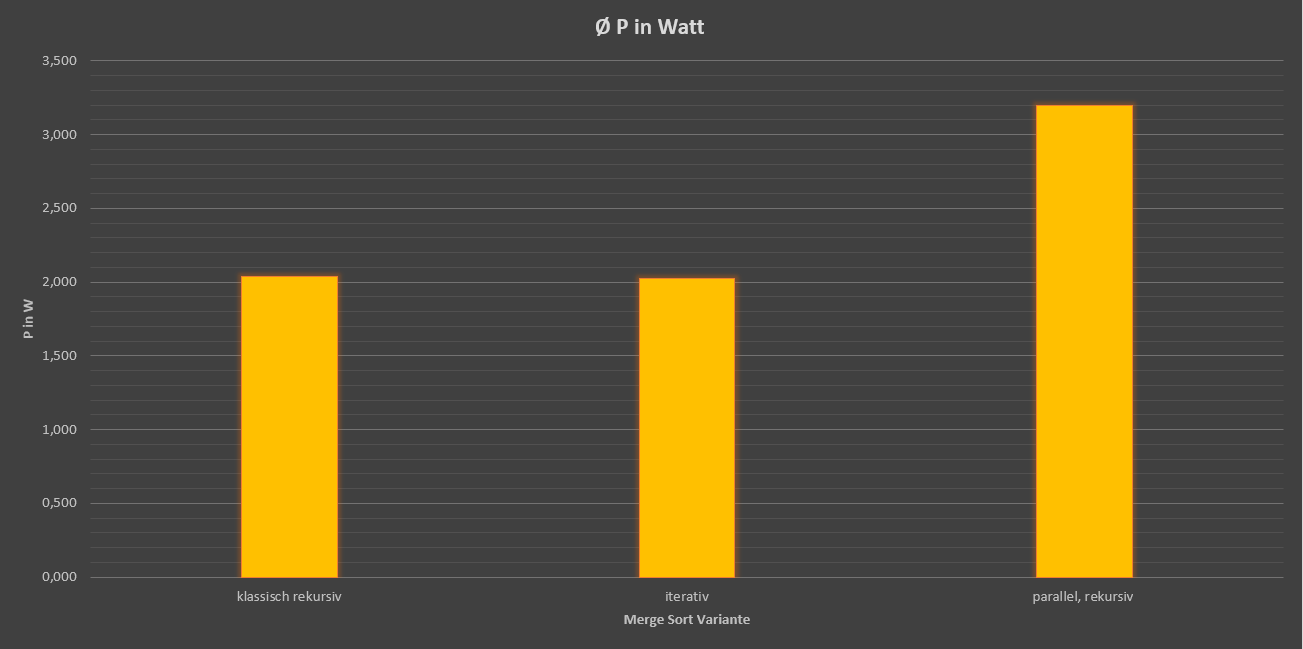
\includegraphics[width=0.8\textwidth]{MergeSortLeistungPic}
	\caption{Merge Sort: durchschnittliche elektrische Leistung pro Verfahren (eigene Abbildung)}
	\label{fig:MergeSortLeistungPic} 
	\end{center}
\end{figure}

% Table generated by Excel2LaTeX from sheet 'Tabelle1'
\begin{table}[htbp]
  \centering
  \caption{elektrische Arbeit und Laufzeit der Merge Sort Varianten Gegen\"uberstellung}
    \begin{tabular}{lrr}
    \toprule
    Merge Sort Variante & \multicolumn{1}{l}{t in s} & \multicolumn{1}{l}{W in Ws} \\
    \midrule
    rekursiv & 804,252 & 1662,462 \\
    \midrule
    iterativ & 714,388 & 1471,137 \\
    \midrule
    parallel & 284,021 & 979,787 \\
    \bottomrule
    \end{tabular}%
  \label{tab:MergeSortLaufzeitArbeit}%
\end{table}%


\begin{figure}[H]
	\begin{center}	 
	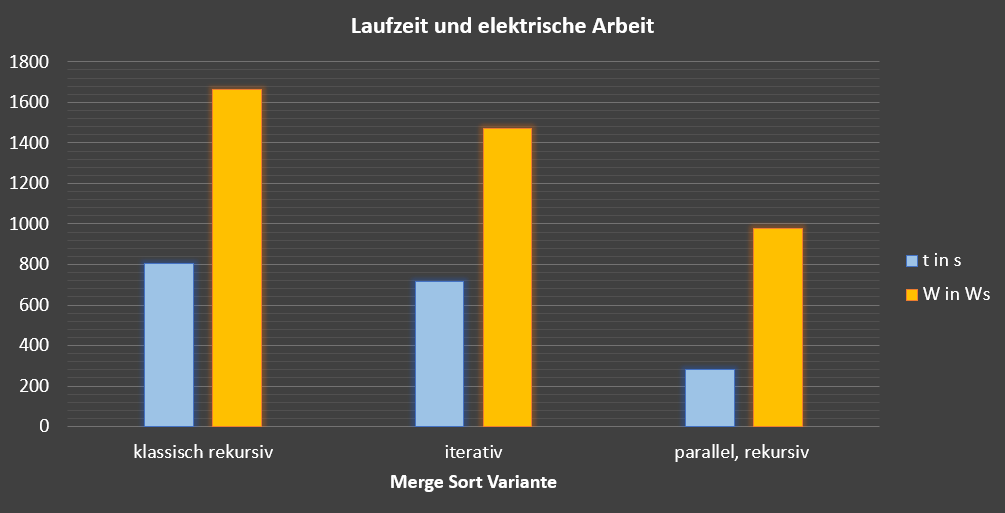
\includegraphics[width=0.8\textwidth]{MergeSortLaufzeitArbeitPic}
	\caption{Merge Sort: Gegenüberstellung von Laufzeiten und elektrischer Arbeit (eigene Abbildung)}
	\label{fig:MergeSortLaufzeitArbeitPic} 
	\end{center}
\end{figure}

\section{Auswertung}